\documentclass{math}

\usepackage{enumerate}
\usepackage{graphicx}

\title{Intro to Computer Science Theory: Homework 9}
\author{Alvin Lin and Joshua Cotton}
\date{August 2017 - December 2017}

\begin{document}

\maketitle

\subsection*{Problem 1}
Give CFGs for the following languages.

\subsection*{Problem 2}
Give state transition diagrams for PDAs for the following languages.
\begin{enumerate}[(a)]
  \item \( \{x\in\{a,b\}^*\mid n_a(x) = n_b(x)\} \)
  \begin{center}
    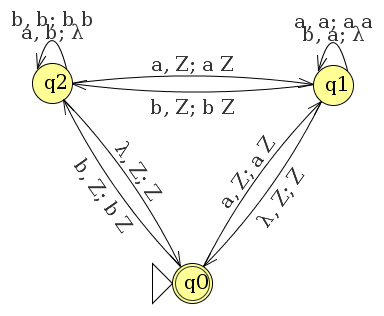
\includegraphics[width=8cm]{assets/hw_9_2a.png}
  \end{center}
  \item \( \{x\in\{a,b\}^*\mid n_b(x)\le n_a(x)\le 2n_b(x)\} \)
  \item The set of all balanced parentheses.
  \begin{center}
    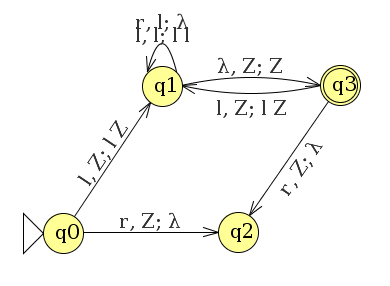
\includegraphics[width=8cm]{assets/hw_9_2c.png}
  \end{center}
\end{enumerate}

\begin{center}
  If you have any questions, comments, or concerns, please contact me at
  alvin@omgimanerd.tech
\end{center}

\end{document}
